% This is samplepaper.tex, a sample chapter demonstrating the
% LLNCS macro package for Springer Computer Science proceedings;
% Version 2.20 of 2017/10/04
%
\documentclass[runningheads]{llncs}
%
\input{solidity-highlighting.tex}

\usepackage{graphicx}\usepackage{tikz,listings,proof}
\usepackage{amssymb}
\usepackage{stmaryrd}
\usetikzlibrary{positioning,shapes,chains}
\usetikzlibrary{shapes.multipart}
\usetikzlibrary[calc]
% Used for displaying a sample figure. If possible, figure files should
% be included in EPS format.
%
% If you use the hyperref package, please uncomment the following line
% to display URLs in blue roman font according to Springer's eBook style:
% \renewcommand\UrlFont{\color{blue}\rmfamily}
\newcommand{\nxt}{\succ}
\newcommand{\revert}{\blacksquare}
\newcommand{\ifs}[3]{\textbf{if}~#1~\textbf{then}~#2~\textbf{else}~#3}
\newcommand{\whiles}[2]{\textbf{while}~#1~\textbf{do}~#2}
\newcommand{\trans}{\triangleright}
\newcommand{\rname}[1]{\textsc{#1}}
\newcommand{\lstate}{\sigma}
\newcommand{\gstate}{\mathtt{\Sigma}}
\newcommand{\conf}[1]{\langle #1 \rangle}
\newcommand{\eval}[1]{\llbracket #1 \rrbracket}
\newcommand{\gas}{\mathcal{G}}
\newcommand{\chain}{\mathbb{B}}
\newcommand{\cstate}{\mathtt{\Gamma}}
\newcommand{\subg}{\stackrel{\ominus}{\leftarrow}}
\newcommand{\addg}{\stackrel{\oplus}{\leftarrow}}
\newcommand{\trace}[2]{\mathsf{trace}(#1,#2)}
\begin{document}
%
\title{Formal Specification for Detecting Vulnerabilities of Ethereum Smart Contracts}
%
%\titlerunning{Abbreviated paper title}
% If the paper title is too long for the running head, you can set
% an abbreviated paper title here
%
\author{}
%
\authorrunning{}
% First names are abbreviated in the running head.
% If there are more than two authors, 'et al.' is used.
%
%\institute{Princeton University, Princeton NJ 08544, USA \and
%Springer Heidelberg, Tiergartenstr. 17, 69121 Heidelberg, Germany
%\email{lncs@springer.com}\\
%\url{http://www.springer.com/gp/computer-science/lncs} \and
%ABC Institute, Rupert-Karls-University Heidelberg, Heidelberg, Germany\\
%\email{\{abc,lncs\}@uni-heidelberg.de}}
%
\maketitle              % typeset the header of the contribution
%
\begin{abstract}
The task of detecting vulnerabilities in Ethereum smart contracts is critical as it protects smart-contract users from losing money due to adversarial exploitation. However, most vulnerabilities are described informally through their syntax rather than the harmful behaviors caused by them. Consequently, this gives rise to many false alarms for the tools that try to detect the bugs due to the mismatches in semantics. In this work, we propose a formal specification language for smart contracts that
 precisely characterizes the vulnerable behaviors via both syntactic and semantics level. We then develop a framework that can verify whether a smart contract is susceptible to the respective vulnerable specification. To evaluate the framework, we implement a C++ tool and use it to detect vulnerabilities of smart contracts on the Ethereum platform.
\keywords{First keyword  \and Second keyword \and Another keyword.}
\end{abstract}

\section{Introduction}

\begin{figure}
\begin{lstlisting}[language=Solidity]
contract Money {
 ...
 function withdraw() {
  assert (msg.sender.call.value(balances[msg.sender])());
  balances[msg.sender] = 0;
 }
}
\end{lstlisting}

\begin{lstlisting}[language=Solidity]
contract Attacker {
 ...
 function() payable{
  if (money.balance >= msg.value) {
   money.withdraw();
  }
 }
}
\end{lstlisting}
\caption{Example of reentrancy attack.}\label{fig:ex1}
\end{figure}

Consider the Solidity function in Fig.~\ref{fig:ex1} in which the sender attempts to withdraw his Ethers recorded in $\texttt{balances[{\color{violet}msg.sender}]}$. The function first tries to conduct the transfer at line 2 in which an Ether amount of $\texttt{balances[{\color{violet}msg.sender}]}$ is sent to the address of the sender, ${\color{violet} \texttt{msg.sender}}$. If the transfer fails (\emph{e.g.} due to insufficient gas) then the transaction is reverted as shown at line 3. Otherwise it is successful and \texttt{balances[{\color{violet}msg.sender}]}---the balance of the sender---is set to 0 at line 4. 

This contract is exposed to the reentrancy attack as the attacker can invoke $\texttt{withdraw}$ multiple times before his balance is set to 0, therefore allows him to withdraw more Ethers than he should. To see why, note that the $\color{blue}\texttt{call}$ function (line 2) also activates the fallback function of $\texttt{msg.sender}$. This allows him to call $\texttt{withdraw}$ from $\texttt{Money}$ contract again as long as the condition $\texttt{money.balance >= msg.value}$ is still satisfiable. Consequently, the Ethers in $\texttt{Money}$ are drained in just a single transaction.

To see how our technique can detect such vulnerability , let 
\\
$$P = \texttt{msg.sender.call.value(balances[msg.sender])()}$$
$$
a = \texttt{throw}~~~~b = \texttt{balances[msg.sender] = 0}
$$

then the function $\texttt{withdraw}$ can be transformed into the following trace set:
$$
T = \mathcal{F}[\textbf{assert}(P)[\textbf{assert}(Q) \cdot \mathcal{F}[T_1]+\textbf{assert}(!Q)] \cdot a]
$$
where $T_1 = \textbf{assert}(P)[\textbf{assert}(Q) \cdot \mathcal{F}+\textbf{assert}(!Q)] \cdot a$. On the other hand, the reentrancy bug is expressed by the following trace:
$$
t = \mathcal{F}[t_1 \cdot \{R_1\}c[t_2 \cdot \mathcal{F}[t_3] \cdot t_4]\{R_2\} \cdot t_5]
$$
where  $t_i$ is trace variable and  $c$ is a basic statement that contains $\textbf{call}$ function. To check whether $\textbf{withdraw}$ is vulnerable under reentrancy, we check whether the word equation $t = T$ has a solution. Indeed, one solution is $t_1 = \epsilon$, $c = \textbf{assert}(P)$, $t_2 = \textbf{assert}(Q)$, $t_3 = \textbf{assert}(P)[\textbf{assert}(!Q)] \cdot a$, $t_4 = \epsilon$, $t_5 = a$. Put everything together, we arrive at:
$$
t' = \mathcal{F}[\textbf{assert}(P)[\textbf{assert}(Q) \cdot \{R_1\}\mathcal{F}[\textbf{assert}(P)[\textbf{assert}(!Q)] \cdot a\{R_2\}]] \cdot a]
$$

We then checking whether the above trace is satisfiable. This can be done by checking the following SAT constraint:
\\
\\
Initial condition:
$$
\texttt{msg.sender0} = \texttt{attacker}
$$
\textbf{assert}(P):
$$
\texttt{money.balance1} = \texttt{money.balance0} - \texttt{balances[msg.sender0]}
$$
$$
\texttt{msg.sender.balance1} =  \texttt{msg.sender.balance0} + \texttt{balances[msg.sender0]}
$$
$$
\texttt{msg.value1} = \texttt{balances[msg.sender0]}
~~~~~
\texttt{msg.sender1} = \texttt{money}
$$
\textbf{assert}(Q):
$$
\texttt{money.balance}_1 >= \texttt{msg.value}_1
$$
$\{R_1\}$:
$$
\texttt{money.balance}_1 = \texttt{a}  > 0
$$
\textbf{assert}(P) (inner):
$$
\texttt{money.balance}_2 = \texttt{money.balance}_1 - \texttt{balances[msg.sender]}_0
$$
$$
\texttt{msg.sender.balance}_2 =  \texttt{msg.sender.balance}_1 + \texttt{balances[msg.sender]}_0
$$
$$
\texttt{msg.value}_2 = \texttt{balances[msg.sender]}_0~~~~~~
\texttt{msg.sender}_2 = \texttt{money}
$$
\textbf{assert}(!Q):
$$
\texttt{money.balance}_2 < \texttt{msg.value}_2
$$
$a:$
$$
\texttt{balances[msg.sender]}_1 = 0
$$
$\{R_2\}$:
$$
\texttt{money.balance}_2 < \texttt{a}
$$
$$
\texttt{msg.sender3} = \texttt{attacker}
$$
$a:$
$$
\texttt{balances[msg.sender3]} = 0
$$



\section{Formalism of traces}

\begin{definition}
A trace set $T$ is called a $n$-approximation of a program $c$ if $c\triangleright_{n}T$ where the relation $\triangleright_{n}$ is defined as:
$$
\infer[{[\rname{base}]}]{c \trans_{n} c}{
	\begin{array}{c}
	\textsf{primitive}(c)
	\end{array}}
~~~~~
\infer[{[\rname{if}]}]{\ifs{b}{c_1}{c_2} \trans_{n} \textbf{assert}(b);t_1+\textbf{assert}(!b);t_2}{c_1 \trans_{n} t_1~~~~ c_2 \trans_{n} t_2}
$$
$$
\infer[{[\rname{while}]}]{\whiles{b}{c} \trans_{n} (\textbf{assert}(b);t)^*;\textbf{assert}(!b)}{c \trans_{n} t}
~~~~~~
\infer[{[\rname{seq}]}]{c_1;c_2 \trans_{n} t_1 ; t_2}{c_1 \trans_{n} t_1~~~~ c_2 \trans_{n} t_2}
$$
$$
\infer[{[\rname{limit}]}]{c_f \trans_{0} c_f}{}~~~~~
\infer[{[\rname{scope}]}]{c_f \trans_{n} c_f[t]}{n > 0~~\textsf{lookup}(c_f) = c~~~c \trans_{n-1} t}
$$	
\end{definition}

\begin{proposition}
	The relation $\triangleright$ satisfies the following properties:
	\begin{enumerate}
		\item $\triangleright_n$ is functional:
		$$
		\forall T_1,T_2.~c \triangleright_n T_1 \Rightarrow c \triangleright_n T_2 \Rightarrow T_1 = T_2
		$$
		\item \textbf{Soundness}: If $c \triangleright_n T$, $t \in T$, $\conf{t,\cstate} \stackrel{*}{\leadsto} \conf{c_{\mathbb{F}},\cstate'}$ then $\conf{c,\cstate} \stackrel{*}{\leadsto} \conf{c_{\mathbb{F}},\cstate'}$.
		\item \textbf{Completeness}: If $\conf{c,\cstate} \stackrel{*}{\leadsto} \conf{c_{\mathbb{F}},\cstate'}$ then there exist $n$, $t$, $T$ s.t.:
		$$c \triangleright_n T \wedge t \in T \wedge \conf{t,\cstate} \stackrel{*}{\leadsto} \conf{c_{\mathbb{F}},\cstate'}$$
	\end{enumerate}
	\end{proposition}
\begin{definition}
	A trace $t$ is concrete if every $c_f$ of it has a scope. A trace $t$ is abstract if it contains variables or guarded conditions.
	\end{definition}

\begin{definition}
	$\eval{c} = \{c\}$, $\eval{t_1+t_2} = \eval{t_1} \cup \eval{t_2}$, $\eval{t^*} = \bigcup_{i=0}^\infty \eval{t^i}$, $\eval{c_f[t]} = \{c_f\} \cup \{c_f[s] \textrm{ s.t. } s \in \eval{t}\}$, $\eval{t_1 \cdot t_2} = \{s_1 \cdot s_2 \textrm{ s.t. } s_1 \in \eval{t_1} \wedge s_2 \in \eval{t_2}\}$ 
	\end{definition}



\section{Specification language}
\subsection{The language}
\begin{figure}
$
\begin{array}{lcl}
\textit{msg}&::=~&\textbf{msg}.\textbf{sender}~|~\ldots~|~\textbf{block}.\textbf{number}~|~\ldots~|~\textbf{now}~|~\textbf{tx}.\textbf{gasprice}~|~\textbf{tx.origin}\\
e&::=~&\textit{msg}~|~\mathbb{Z}~|~\textit{var}~|~\textbf{address}~|~\textbf{balance}~|~c_f~|~\textit{arr}[e]~|~\textit{arr}.\textbf{length}~|~e + e~|~ \ldots\\
b&::=~&\textbf{true}~|~\textbf{false}~|~c_f~|~ e = e~|~ e < e~|~e \leq e ~|~ !b~|~ b \&\& b  ~|~ b || b
\\
c_b&::=~&\textit{primitive}~|~\textbf{continue}~|~\textbf{break}~|~\textbf{return}~e~|~\textbf{assert}(b)~|~\textbf{require}(b)~|~\textbf{throw}\\
c_f&::=~&f(\bar{e})~|~\textit{addr}.f(\bar{e})~|~\textit{addr}.\textbf{call}(f,\bar{e}).\textbf{gas}(e_g).\textbf{value}(e_v)~|~\\
&&\textit{addr}.\textbf{delegatecall}(f,\bar{e}).\textbf{gas}(e_g)~|~\textit{addr}.\textbf{send}(e)~|~\textit{addr}.\textbf{transfer}(e)\\
c&::=~&c_b~|~c_f~|~c;c~|~\ifs{b}{c}{c}~|~\whiles{b}{c}
\end{array}
$
\caption{A light-weight language for Solidity}\label{fig:lang}
\end{figure}


We adopt the light-weight language in Fig.~\ref{fig:lang} to specify Solidity functions. The first constructor $\textit{msg}$ contains transaction global variables such as $\textbf{msg.sender}$---the address of the sender, $\textbf{block.number}$---the transaction's block number, or $\textbf{now}$---the transaction's time stamp, \emph{etc}. The constructor $e$ captures the syntax for arithmetic expressions including $\textit{msg}$, integers $\mathbb{Z}$, variables $\textit{var}$, the \textbf{address} and \textbf{balance} of the current contract, function call $c_f$, together with standard arithmetic operations. Similarly, the constructor $b$ is for writing Boolean expressions such as truth values $\{\textbf{true},\textbf{false}\}$, function call $c_f$, array access $\textit{arr}[e]$ and its length $\textit{arr}.\textbf{length}$, expression comparisons $\{e=e,e < e,e \leq e\}$, together with Boolean connectives $\{!,\&\&,||\}$. 


Next we have $c_b$ for basic statements such as primitive commands (\textbf{skip}, assignment $x:=e$, \ldots), flow control $\{\textbf{continue},\textbf{break},\textbf{return}\}$,  error check $\{\textbf{assert},\textbf{require}\}$, and exception raise $\textbf{throw}$. The constructor $c_f$ is for function calls such as internal call $f(\bar{e})$ and external call $\textit{addr}.f(\bar{e})$ where $\textit{addr}$ is the external contract's address, $f$ is the function id, and $\bar{e}$ is the argument list. For external calls, the fallback function is executed by default if no function can match the signature $(f,\bar{e})$. Here fallback is a special function in Solidity contracts that has no name and receives no argument. Another external calls is $\textit{addr}.\textbf{call}(f,\bar{e}).\textbf{gas}(e_g).\textbf{value}(e_v)$ which is low-level. By design, low-level calls in Solidity do not propagate exceptions or return values to their callers, instead a Boolean value is returned in which $\textbf{false}$ is equivalent to the occurrence of an exception. When the above $\textbf{call}$ is executed, the current contract sends an amount of $e_v$ Ether to address $\textit{addr}$. At the same time, it also provides a gas stipend of $e_g$ Ether to execute the function $f$ at $\textit{addr}$ with arguments $\bar{e}$. On the other hand, the low-level external call $\textit{addr}.\textbf{delegatecall}(f,\bar{e}).\textbf{gas}(e_g)$ possesses similar behaviors as $\textbf{call}$ except there is no context switching between the caller and the callee. This means the function $f$ is executed in the current contract's context instead of the $\textit{addr}$'s context, thus the field $\textbf{value}$ is redundant and omitted.  The two statements $\textit{addr}.\textbf{send}(e)$ and $\textit{addr}.\textbf{transfer}(e)$ behave similarly as both send an amount of $e$ Ether to address $\textit{addr}$, together with a gas stipend of $2300$ wei to execute the fallback function at address  $\textit{addr}$. However, $\textbf{send}$ is low-level and thus it cannot propagate exceptions like $\textbf{transfer}$.  Finally, we have constructor $c$ for general statements which consists of basic statements $c_b$, function calls $c_f$, composition $c;c$, conditional statement $\ifs{b}{c}{c}$, and while loop $\whiles{b}{c}$.

Note that we focus on the high-level semantics of Solidity and thus our light-weight language do not support the full spectrum of data types and structures in Solidity such as bytes, struct, object, String. For simplicity, we also exclude the statement $\textbf{for}(c_1;b;c_2)\{c\}$ from our language since it can be equivalently transformed into the while statement $c_1;\whiles{b}{\{c;c_2\}}$.
\begin{figure}
$
\begin{array}{lcl}
\mathsf{e}&::=~&\overline{\textit{symbolic}}~|~\textit{const}~|~\textit{var}~|~c_f~|~\textit{id}.f(\bar{\textsf{e}})~|~\mathsf{e} + \mathsf{e}~|~ \mathsf{e} - \mathsf{e}~|~ \mathsf{e} \times \mathsf{e} ~|~ \mathsf{e}~\textbf{div}~\mathsf{e}~|~ \mathsf{e}~\textbf{mod}~\mathsf{e}\\
\textit{mod}&::=~&\textsf{owned}~|~ \textsf{public}~|~\textsf{private}~|~\textsf{payable}~|~\textsf{pure}~|~\textsf{view}~|~\textsf{external}\\
P&::=~&\textbf{true}~|~\textbf{false}~|~\textit{mod}~|~ \mathsf{e} = \mathsf{e}~|~ \mathsf{e} < \mathsf{e}~|~\ldots~|~!P~|~P \&\& P ~|~ P || P ~|~ \exists x.~P~|~ \forall x.~P\\
t&::=~&c_{p}~|~c_f~|~\{P\}t~|~t\{P\}~|~c_f[t]~|~t \nxt t~|~t+t~|~t^*\\
T&::=~&\emptyset~|~a~|~\{P\}T~|~T\{P\}~|~\overline{c_f}~|~\overline{c_f}[T]~|~T \nxt T~|~T\cup T~|~T \cap T ~|~T^*\\
\kappa&::=~&v~|~c~|~\conf{\kappa}~|~\conf{\kappa,\cstate}~|~\kappa ; \kappa
\end{array}
$
\caption{Assertion language and trace definition}\label{fig:assert}
\end{figure}

\subsection{Vulnerabilities}


Note: we don't support cross-transaction traces, \emph{i.e.} traces with functions executed in different transactions. Need an invariant for state that says "all variables's values are the same", can simply over-approximate to variables in the functions.
\begin{enumerate}
	\item Integer overflow/underflow:
	$$
	\mathcal{F}[\overline{t_1} \nxt \{x \geq \textit{min}\}\overline{t_2}\{x < \textit{min}\} \nxt \overline{t_3}]
	~~~~~
	\mathcal{F}[\overline{t_1} \nxt \{\overline{x} \leq \textit{max}\}\overline{t_2}\{\overline{x} > \textit{max}\} \nxt \overline{t_3}]
	$$
	where $\overline{t_2} \in \{e:= e + e, e:= e - e, e:= e \times e, e:= e~\textbf{div}~e\}$
	\item Unchecked send:
	$$
	\mathcal{F}[\overline{t_1} \nxt \overline{\textit{addr}}.f \nxt \overline{t_2}]
	$$
	
	where $f \in \{\textbf{send},\textbf{transfer},\textbf{call}\}$
	\item Reentrancy:
	$$
	\mathcal{F}[\{\textbf{balance} = \overline{a_0}\}\overline{t_1} \nxt \overline{\textit{addr}}.\textbf{call}.\textbf{value}(\overline{v}).()[\mathcal{F}[\overline{t_2}\{\textbf{balance} < \overline{a_0}\}]] \nxt \overline{t_3}]
	$$
	
	\item Suicide contracts:
	$$
	\mathcal{F}[\{!\textsf{owned}\}\overline{t_1} \nxt \textbf{selfdestruct}(\overline{\textit{addr}}) \nxt \overline{t_2}]
	$$
	\item Time-stamp dependency:
	$$
\mathcal{F}[\overline{t_1} \nxt a \nxt \overline{t_2}]
$$

where $a$ is a primitive statement that contains the $\textbf{now}$ keyword

	\item Block dependency:
	$$
	\mathcal{F}[\overline{t_1} \nxt a \nxt \overline{t_2}]
	$$
	
	where $a$ is a primitive statement that contains the $\textbf{block}.\textbf{number}$ keyword
	
	
	\item Transaction ordering dependency:
	$$
	\overline{\textit{addr}}.\textit{atk}(\{x = \overline{x_0}\}\mathcal{F}_1 \nxt \mathcal{F}_2\{x = \overline{x_1}\}) \cap \{x = \overline{x_0}\}\mathcal{F}_2  \nxt \mathcal{F}_1 \{x = \overline{x_2}\}
	$$
	
	where $x_1 \neq x_2$
	\item Unsafe delegatecall:
	$$
	\mathcal{F}[\overline{t_1} \nxt \overline{\textit{addr}}.\textbf{delegatecall}(\textbf{msg.data}) \nxt \overline{t_2}]
	$$
\end{enumerate}

Let $\lstate$ be the local state and $\gstate$ be the global state. A local configuration is the tuple $\conf{c,\lstate,\gstate}$ of statement, local state and global state. A small step is a binary between two configurations: $\conf{c,\lstate,\gstate} \leadsto \conf{c',\lstate',\gstate'}$. We provide the following sequential operational semantics where $\cstate = \conf{\lstate,\gstate,\chain,b}$:

\begin{figure}
$$
\infer[{[\rname{txs}]}]{\conf{m{::}M,\chain} \leadsto \conf{M,\chain'}}
{
	\begin{array}{c}
	m = (\gstate,\textit{addr})~~~\gstate.\textbf{msg} = (s,v,f,\bar{a})~~~ \chain(\textit{addr}) = (\mathcal{C},\lstate)~~~\mathcal{C}(f,\bar{a}) = c\\
	\chain_1 = \chain[s \stackrel{v}{\rightarrow} \textit{addr}]~~~
	\cstate = (\lstate,\gstate,\chain_1,\textbf{false})~~~
	\conf{c,\cstate} \stackrel{*}{\leadsto} \conf{c_\mathbb{F},\cstate'}~~~
	\chain' = \cstate'.\chain
	\end{array}
}
$$

$$
\infer[{[\rname{txf}]}]{\conf{m{::}M,\chain} \leadsto \conf{M,\chain}}
{
	\begin{array}{c}
	m = (\gstate,\textit{addr})~~~\gstate.\textbf{msg} = (s,v,f,\bar{a})~~~ \chain(\textit{addr}) = (\mathcal{C},\lstate)~~~\mathcal{C}(f,\bar{a}) = c\\
	\chain_1 = \chain[s \stackrel{v}{\rightarrow} \textit{addr}]~~~~~
	\cstate = (\lstate,\gstate,\chain_1,\textbf{false})~~~~~
	\conf{c,\cstate} \stackrel{*}{\leadsto} \conf{\textbf{throw},\cstate'}
	\end{array}
}
$$
\caption{Transaction semantics}\label{fig:tx}
\end{figure}

\subsection{Notations for semantics}

We first introduce several notations to help define the semantics.  A \emph{message} $m$ is a pair $(\gstate,\textit{addr})$ of the message state $\gstate$ and the receiver's address $\textit{addr}$. Here the message state $\gstate$ is represented by the quadruple $(s,v,f,\bar{a})$ that consists of the sender's address $s$, the Ether value $v$ of the transaction, the method id $f$ together with inputs $\bar{a}$ to be called at the receiver's address. A ledger $\chain$ is a finite mapping from addresses to pairs of contract code $\mathcal{C}$ and its state $\lstate$. The method's code in contract $\mathcal{C}$ can be accessed by providing the method id and its parameter, \emph{e.g} $\mathcal{C}(f,\bar{a})$. A transaction step $\stackrel{t}{\leadsto}$ relates two transaction configurations (t-config), \emph{e.g.} $\conf{M,\chain} \stackrel{t}{\leadsto} \conf{M',\chain'}$ where each t-config is a pair of message list and ledger. 

At the contract level we have contract step $\leadsto$ that relates two contract configurations (c-config), \emph{e.g.} $\conf{\kappa,\cstate} \leadsto \conf{\kappa',\cstate'}$ where each c-config is a pair of \emph{activation record} $\kappa$ and \emph{transaction state} $\cstate$. The activation record $\kappa$ can be either a concrete value $v$, a statement $c$, a \emph{scoped statement} $\conf{c}$ (for bookkeeping the scopes of $\textbf{continue}$ and $\textbf{break}$), a pair of activation record and transaction state $\conf{\kappa',\gstate'}$ (for bookkeeping the scopes of function calls), an evaluating assignment $x:= \conf{\kappa',\gstate'}$, or a composition of two activation records $\kappa_1;\kappa_2$. An activation record $\kappa$ is \emph{final} if it is $\textbf{skip}$ or some concrete value $v$. For convenience, we use $\kappa_{\mathbb{F}}$ to represent final activation records. The transaction state $\cstate$ is expressed by the quadruple $(\lstate,\gstate,\chain,b)$ of contract state $\lstate$, message state $\gstate$, ledger $\chain$, and Boolean flag $b$ (for bookkeeping exception propagation).


We also introduce several notations for updating the states. The action $\beta$ for a state $s$ (\emph{i.e.} ledger $\chain$, message $\gstate$, contract $\lstate$) is written as $s[\beta]$. Here action can be updating a variable, \emph{i.e.} $s[x \leftarrow v]$ means the variable $x$ in $s$ is updated with new value $v$. Or the action can be Ether transfer between two addresses, \emph{i.e.} $\chain[\textit{addr}_1 \stackrel{v}{\rightarrow} \textit{addr}_2]$ indicates the transfer of $v$ Ethers from $\textit{addr}_1$ to $\textit{addr}_2$. 

\begin{figure}[t]
\centering
$$
\infer[{[\rname{sk}]}]{\conf{c;c',\cstate} \leadsto \conf{c',\cstate}}{c \in \mathbb{V} \cup \{\textbf{skip},\textbf{continue},\textbf{break}\}}
~~~~~~
\infer[{[\rname{er}]}]{\conf{c,\cstate} \leadsto \conf{\textbf{throw},\cstate}}{\textit{error}}
~~~~~~
\infer[{[\rname{th}]}]{
	\begin{array}{c}
	\conf{\textbf{throw};c,\cstate}
	\leadsto \conf{\textbf{throw},\cstate}
	\end{array}
	}{}
$$

$$
\infer[{[\rname{as}]}]
{
	\begin{array}{l}
	\conf{x:=e,\cstate} 
	\leadsto \conf{\textbf{skip},\cstate'}
	\end{array}
}{
	\begin{array}{c}
	\eval{e}_{\cstate} = (v,\cstate_1)
	\\
	\cstate' = \cstate_1[\lstate.x \leftarrow v][\gstate.\textbf{gas} \subg \gas(:=)]
	\end{array}}
~~~
\infer[{[\rname{re}]}]{
	\begin{array}{c}
		\conf{\textbf{return}~e;c, \cstate}
		\leadsto \conf{v,\cstate'}
	\end{array}
}{\eval{e}_\cstate  = (v,\cstate')}
~~~
\infer[{[\rname{seq}]}]{
	\begin{array}{c}
		\conf{c_1;c_2,\cstate}
		\leadsto \conf{c'_1;c_2,\cstate'}
	\end{array}
}{\conf{c_1,\cstate} \leadsto \conf{c'_1,\cstate'}}	
$$

$$
\infer[{[\rname{at}]}]{\conf{c(b),\cstate} \leadsto \conf{\textbf{skip},\cstate'}}{
	\begin{array}{c}
	c \in \{\textbf{require},\textbf{assert}\}
	~~~~~
	\eval{b}_{\cstate} = (\textbf{true},\cstate')
	\end{array}
}
~~~~~~
\infer[{[\rname{af}]}]{\conf{c(b),\cstate} \leadsto \conf{\textbf{throw},\cstate'}}{
	\begin{array}{c}
	c \in \{\textbf{require},\textbf{assert}\}~~~
	~~~~~
	\eval{b}_{\cstate} = (\textbf{false},\cstate')
	\end{array}}
$$

$$
\infer[{[\rname{it}]}]{
	\begin{array}{c}
	\conf{\ifs{b}{c_1}{c_2},\cstate}
	\leadsto \conf{c_1,\cstate'}
	\end{array}
}
{
	\begin{array}{c}
	\eval{b}_{\cstate} = (\textbf{true},\cstate')
	\end{array}
}	
~~~~~~
\infer[{[\rname{if}]}]{
	\begin{array}{c}
	\conf{\ifs{b}{c_1}{c_2},\cstate}
	\leadsto \conf{c_2,\cstate'}
	\end{array}
}
{
	\begin{array}{c}
	\eval{b}_{\cstate} = (\textbf{false},\cstate')\\
	\end{array}
}	
$$

$$
\infer[{[\rname{wt}]}]
{
	\begin{array}{c}
	\conf{\whiles{\textbf{true}}{c},\cstate}
	\\
	 \leadsto \conf{\conf{c};\whiles{b}{c},\cstate'}
	\end{array}
}
{
	\begin{array}{c}
	\eval{b}_{\cstate} = (\textbf{true},\cstate')
	\end{array}
}
~~~~~
\infer[{[\rname{wf}]}]
{
	\begin{array}{c}
	\conf{\whiles{b}{c},\cstate} \\
	\leadsto
	\conf{\textbf{skip},\cstate'}
	\end{array}
}
{
	\begin{array}{c}
	\eval{b}_{\cstate} = (\textbf{false},\cstate')
	\end{array}
}
~~~~
\infer[{[\rname{bk}]}]{
	\begin{array}{c}
	\conf{\conf{\textbf{break};c};\whiles{b}{c'},\cstate} 
	\\
	\leadsto \conf{\textbf{skip},\cstate}
	\end{array}
}{
}
$$

$$
\infer[{[\rname{ct}]}]{
	\begin{array}{c}
	\conf{\conf{\textbf{continue};c},\cstate}
	\leadsto \conf{\textbf{skip},\cstate}
	\end{array}
}{}
~~~~
\infer[{[\rname{in}]}]{\conf{\conf{c_1;c_2},\cstate} \leadsto \conf{\conf{c_1';c_2},\cstate'}}
{
	\begin{array}{c}
	c_1 \not \in \{\textbf{continue},\textbf{break}\}
	\\
	\conf{c_1,\cstate} \leadsto \conf{c_1',\cstate'}
	\end{array}
}
~~~~
\infer[{[\rname{out}]}]{\conf{\conf{c},\cstate} \leadsto \conf{c,\cstate}}{ c \in \mathbb{V} \cup \{\textbf{skip},\textbf{throw}\}}
$$
\caption{Operational semantics for basic commands.}\label{fig:opbasic}
\end{figure}

\begin{figure}[t]
\centering
$$
\infer[{[\rname{ifun}]}]{\conf{f(\bar{a}),\cstate} \leadsto \conf{\conf{c_f,\cstate_f},\cstate'}}
{
	\begin{array}{c}	
	\eval{\bar{a}}_{\cstate} = (\bar{v},\cstate_1)~~~
	\cstate_1.\mathbb{B}(\lstate.\textit{addr}) = (\mathcal{C}_f,\lstate_f)~~~~
	\mathcal{C}_f.f = (c_f,\overline{s})~~~\lstate_f' = \lstate_f[\overline{s} \leftarrow \overline{v}]
	\\
	\cstate_f = \cstate_1[\lstate \leftarrow \lstate_f'][b \leftarrow \textbf{false}]~~~
	\cstate' = \cstate_1[\gstate.\textit{gas}  \leftarrow 0]
	\end{array}
}
$$
$$
\infer[{[\rname{fun}]}]{\conf{\textit{addr}.f(\bar{a}),\cstate} \leadsto \conf{\conf{c_f,\cstate_f},\cstate'}}
{
	\begin{array}{c}	
	\eval{\bar{a}}_{\cstate} = (\bar{v},\cstate_1)~~~
	\cstate_1.\mathbb{B}(\textit{addr}) = (\mathcal{C}_f,\lstate_f)~~~~
	\mathcal{C}_f.f = (c_f,\bar{s})~~~~\lstate_f' = \lstate_f[\overline{s} \leftarrow \overline{v}]
	\\
	\cstate_f = \cstate_1[\gstate.\textit{msg}.\textit{sender} \leftarrow \lstate.\textit{addr}][\lstate \leftarrow \lstate_f'][b \leftarrow \textbf{false}]~~~
	\cstate' = \cstate_1[\gstate.\textit{gas}  \leftarrow 0]
	\end{array}
}
$$
\vspace{-0.5em}
$$
\infer[{[\rname{call}]}]{\conf{\textit{addr}.\textbf{call}(f,\bar{a}).\textbf{value}(e).\textbf{gas}(g),\cstate} \leadsto \conf{\conf{c_f,\cstate_f},\cstate'}}
{
	\begin{array}{c}	
	\eval{(\bar{a},e,g)}_{\cstate} = ((\bar{v},v_e,v_g),\cstate_1)~~~~
	\cstate_1.\mathbb{B}(\textit{addr}) = (\mathcal{C}_f,\lstate_f)
	~~~~\mathcal{C}.f = (c_f,\overline{s})~~~~\lstate_f' = \lstate_f[\overline{s} \leftarrow \overline{v}]
	\\
	\cstate_2 = \cstate_1[\gstate.\textit{msg}.\textit{sender} \leftarrow \lstate.\textit{addr}][\gstate.\textit{msg}.\textit{value} \leftarrow v_e][\gstate.\textit{gas} \leftarrow v_g]
	\\
	\cstate_f = \cstate_2[\chain(\lstate.\textit{addr}) \stackrel{v_e}{\rightarrow} \chain(\textit{addr})][\lstate \leftarrow \lstate_f'][b \leftarrow \textbf{true}]
	~~~~
	\cstate' = \cstate_1[\gstate.\textit{gas} \subg v_g]
	\end{array}
}
$$
\vspace{-0.5em}
$$
\infer[{[\rname{dcall}]}]{\conf{\textit{addr}.\textbf{delegatecall}(f,\bar{a}).\textbf{gas}(g),\cstate} \leadsto \conf{\conf{c_f,\cstate_f},\cstate'}}
{
	\begin{array}{c}	
	\eval{(\bar{a},g}_{\cstate} = ((\bar{v},v_g),\cstate_1)~~~
	\cstate_1.\mathbb{B}(\textit{addr}) = (\mathcal{C}_f,\lstate_f)
	~~~\mathcal{C}_f.f = (c_f,\overline{s})
	\\
	\cstate_f = \cstate_1[\gstate.\textit{gas} \leftarrow v_g][b \leftarrow \textbf{true}]
	~~~
	\cstate' = \cstate_1[\gstate.\textit{gas} \subg v_g]
	\end{array}
}
$$
\vspace{-0.5em}
$$
\infer[{[\rname{tf}]}]{\conf{\textit{addr}.\textbf{transfer}(e),\cstate} \leadsto \conf{\conf{c_f,\cstate_f},\cstate'}}
{
	\begin{array}{c}	
	\eval{e}_\cstate = (v_e,\cstate_1)~~~
	\cstate_1.\mathbb{B}(\textit{addr}) = (\mathcal{C}_f,\lstate_f)~~~~
	\mathcal{C}.() = (c_f,\_)
	\\
	\cstate_2 = \cstate_1[\gstate.\textit{msg}.\textit{sender} \leftarrow \lstate.\textit{addr}][\gstate.\textit{msg}.\textit{value} \leftarrow v_e][\gstate.\textit{gas} \leftarrow 2300]
	\\
	\cstate_f = \cstate_2[\chain(\lstate.\textit{addr}) \stackrel{v_e}{\rightarrow} \chain(\textit{addr})][\lstate \leftarrow \lstate_f][b \leftarrow \textbf{false}]~~~~
	\cstate' = \cstate_1[\gstate.\textit{gas} \subg 2300]
	\end{array}
}
$$
\vspace{-0.5em}
$$
\infer[{[\rname{send}]}]{
	\begin{array}{c}
	\conf{\textit{addr}.\textbf{send}(e),\cstate} \leadsto
	\\
	\conf{\textit{addr}.\textbf{call}((),\_).\textbf{value}(e).\textbf{gas}(2300),\cstate}
	\end{array}
}
{
}
~~~~
\infer[{[\rname{kill}]}]{
	\conf{\textbf{selfdestruct}(\textit{addr}),\cstate} \leadsto \conf{\textbf{skip},\cstate'}
}
{
	\begin{array}{ll}
	\cstate' = \cstate[\chain(\lstate.\textit{addr}) \stackrel{\lstate.\textit{bal}}{\longrightarrow}  \chain(\textit{addr})]
	[\chain(\lstate.\textit{addr}) \leftarrow \textbf{None}]
	\end{array}
}
$$
\vspace{-0.5em}
$$
\infer[{[\rname{run}]}]{\conf{\conf{c_f,\cstate_f},\cstate} \leadsto \conf{\conf{c_f',\cstate_f'},\cstate}}
{
	\begin{array}{c}	
	\conf{c_f,\cstate_f} \leadsto \conf{c_f',\cstate_f'}
	\end{array}
}
~~~~
\infer[{[\rname{cf}]}]{\conf{\conf{\textbf{throw},\cstate_f},\cstate} \leadsto \conf{\textbf{false},\cstate'}}
{
	\begin{array}{c}	
	\cstate.b = \textbf{true}\\
	\cstate' = \cstate[\gstate.\textit{gas} \addg g_f]
	\end{array}
}
~~~~
\infer[{[\rname{ff}]}]{\conf{\conf{\textbf{throw},\cstate_f},\cstate} \leadsto \conf{\textbf{throw},\cstate'}}
{
	\begin{array}{c}	
	\cstate.b = \textbf{false}\\
	\cstate' = \cstate[\gstate.\textit{gas} \addg g_f]
	\end{array}
}
$$
\vspace{-0.5em}
$$
~~~~~~~~~~~~~
\infer[{[\rname{fs}]}]{\conf{\conf{c,\cstate_f},\cstate} \leadsto \conf{c,\cstate'}}
{
	\begin{array}{c}
	c \in \mathbb{V} \cup \{\textbf{skip}\}	~~~~~ \cstate.b = \textbf{false}
	\\
	\cstate_1 = \cstate[\chain \leftarrow \cstate_f.\chain][\gstate.\textit{gas} \addg g_f]
	\\
	\cstate' = \cstate_1[\chain(\cstate_f.\lstate.\textit{addr}) \stackrel{m}{\leftarrow} \cstate_f.\lstate]
	\end{array}
}
~~~~~~
\infer[{[\rname{cs}]}]{\conf{\conf{c,\cstate_f},\cstate} \leadsto \conf{\textbf{true},\cstate'}}
{
	\begin{array}{c}
	c \in \mathbb{V} \cup \{\textbf{skip}\}	~~~~~ \cstate.b = \textbf{true}\\
	\cstate_1 = \cstate[\chain \leftarrow \cstate_f.\chain][\gstate.\textit{gas} \addg g_f]
	\\
	\cstate' = \cstate_1[\chain(\cstate_f.\lstate.\textit{addr}) \stackrel{m}{\leftarrow} \cstate_f.\lstate]
	\end{array}
}
$$
\caption{Operational semantics for function calls.}\label{fig:opfun}
\end{figure}

\begin{figure}
$$
\infer[{[\rname{base}]}]{\conf{\cstate,c,\cstate'} \models \mathcal{A}(c)}{\textit{primitive}(c)~~~\conf{c,\cstate} \leadsto \conf{v,\cstate'}}
~~~~~
\infer[{[\rname{em}]}]{\conf{\cstate,c,\cstate'} \models t}{\conf{c,\cstate} \stackrel{\epsilon}{\leadsto} \conf{c_1,\cstate_1}~~~\conf{\cstate_1,c_1,\cstate'} \models t}
$$

$$
\infer[{[\rname{case}_1]}]{\conf{\cstate,c,\cstate'} \models t_1+t_2}{\conf{\cstate,c,\cstate'} \models t_1}
~~~~~
\infer[{[\rname{case}_2]}]{\conf{\cstate,c,\cstate'} \models t_1+t_2}{\conf{\cstate,c,\cstate'} \models t_2}
$$

$$
\infer[{[\rname{cut}]}]{\conf{\cstate,c_1;c_2;\cstate'} \models t_1 \nxt t_2}{\conf{\cstate,c_1,\cstate_1} \models t_1~~~\conf{\cstate_1,c_2,\cstate'} \models t_2}
~~~~~
\infer[{[\rname{star}_1]}]{\conf{\cstate,c,\cstate'} \models t^*}{\conf{\cstate,c,\cstate'} \models \epsilon}
~~~~~
\infer[{[\rname{star}_2]}]{\conf{\cstate,c,\cstate'} \models t^*}{\conf{\cstate,c,\cstate'} \models t \nxt t^*}
$$

$$
\infer[{[\rname{cond}_1]}]{\conf{\cstate,c,\cstate'} \models \{P\}t}{\conf{\cstate,c,\cstate'} \models t~~~~~\eval{P}_{\cstate} = \textbf{true}}
~~~~~
\infer[{[\rname{cond}_2]}]{\conf{\cstate,c,\cstate'} \models t\{P\}}{\conf{\cstate,c,\cstate'} \models t~~~~~\eval{P}_{\cstate'} = \textbf{true}}
$$



$$
\infer[{[\rname{fun}_1]}]{\conf{\cstate,f,\cstate'} \models \mathcal{F}(f)[t]}
{
	\begin{array}{ll}
	\conf{f,\cstate} \leadsto \conf{\conf{c_f,\cstate_f},\cstate'}
	&~~~\conf{c_f,\cstate_f} \stackrel{*}{\leadsto} \conf{v,\cstate_f'}
	\\
	\conf{\conf{v,\cstate_f'},\cstate} \leadsto \conf{v,\cstate'}
	&~~~\conf{\cstate_f,c_f,\cstate_f'} \models t
	\end{array}
}
~~~~~
\infer[{[\rname{fun}_2]}]{\conf{\cstate,f,\cstate'} \models \mathcal{F}(f)}{\conf{f,\cstate} \stackrel{*}{\leadsto} \conf{v,\cstate'}}
$$
\caption{Trace semantics}\label{fig:trace}
\end{figure}


A trace $t$ is belong to a program $c$, denoted as $t \in \mathbb{T}(c)$, iff for all $\cstate$, $\cstate'$ we have $\conf{t,\cstate} \stackrel{*}{\leadsto} \conf{f,\cstate'}$ implies $\conf{c,\cstate} \stackrel{*}{\leadsto} \conf{f,\cstate'}$ where $\conf{f,\cstate'}$ is final, \emph{i.e.}:
$$
t \in \mathbb{T}(c) ~\stackrel{\triangle}{=}~ \forall \cstate,\cstate',t_{\mathbb{F}}, f.\conf{t,\cstate} \hookrightarrow \conf{t_{\mathbb{F}},\cstate'} \Rightarrow \conf{c,\cstate} \stackrel{*}{\leadsto} \conf{t_{\mathbb{F}},\cstate'}
$$


Evaluation:
\begin{figure}
$$
\infer[\rname{base}]{\conf{t,\cstate} \hookrightarrow \conf{t_{\mathbb{F}},\cstate'}}{\textsf{command}(t)~~~\conf{t,\cstate} \stackrel{*}{\leadsto} \conf{t_{\mathbb{F}},\cstate'}}
~~~
\infer[\rname{left}]{\conf{t_1+t_2,\cstate} \hookrightarrow \conf{t_{\mathbb{F}},\cstate'}}{\conf{t_1,\cstate} \hookrightarrow \conf{t_{\mathbb{F}},\cstate'}}
~~~
\infer[\rname{right}]{\conf{t_1+t_2,\cstate} \hookrightarrow \conf{t_{\mathbb{F}},\cstate'}}{\conf{t_2,\cstate} \hookrightarrow \conf{t_{\mathbb{F}},\cstate'}}
$$

$$
\infer[\rname{pre}]{\conf{\{P\}t,\cstate} \hookrightarrow \conf{t_{\mathbb{F}},\cstate'}}{\eval{P}_\cstate = \textbf{true}~~~\conf{t,\cstate} \hookrightarrow \conf{t_{\mathbb{F}},\cstate'}}
~~~~~
\infer[\rname{post}]{\conf{t\{P\},\cstate} \hookrightarrow \conf{t_{\mathbb{F}},\cstate'}}{\conf{t,\cstate} \hookrightarrow \conf{t_{\mathbb{F}},\cstate'}~~~\eval{P}_{\cstate'} = \textbf{true}}
$$

$$
\infer[\rname{star}_1]{\conf{t^*,\cstate} \hookrightarrow \conf{t_{\mathbb{F}},\cstate'}}{\conf{t \nxt t^*,\cstate} \hookrightarrow \conf{t_{\mathbb{F}},\cstate'}}
~~~~~
\infer[\rname{star}_2]{\conf{t^*,\cstate} \hookrightarrow \conf{\textbf{skip},\cstate}}{}
$$

$$
\infer[\rname{seq}_1]{\conf{t_1 \nxt t_2,\cstate} \hookrightarrow \conf{t_{\mathbb{F}}' ,\cstate'}}{\conf{t_1,\cstate} \hookrightarrow \conf{t_{\mathbb{F}},\cstate_1}~~~\conf{t_2,\cstate_1} \hookrightarrow \conf{t_{\mathbb{F}}',\cstate'}~~~t_\mathbb{F} \neq \textbf{throw}}
~~~~~
\infer[\rname{seq}_2]{\conf{t_1 \nxt t_2,\cstate} \hookrightarrow \conf{\textbf{throw} ,\cstate'}}{\conf{t_1,\cstate} \hookrightarrow \conf{\textbf{throw},\cstate'}}
$$

$$
\infer[\rname{scope}]{\conf{t_f[t],\cstate} \hookrightarrow \conf{t'_{\mathbb{F}},\cstate'}}
{
	\begin{array}{c}
	\conf{t_f,\cstate} \leadsto \conf{\conf{c_f,\cstate_f},\cstate_1}~~~\conf{t,\cstate_f} \hookrightarrow \conf{t_{\mathbb{F}},\cstate_f'}\\
	\conf{\conf{t_{\mathbb{F}},\cstate_f'},\cstate_1} \leadsto \conf{t'_{\mathbb{F}},\cstate'}~~~~~~t_f \in \{f(\bar{a}),\textit{addr}.f(\bar{a})\}
	\end{array}
}
$$
\caption{A trace semantics}\label{fig:tracesem}
\end{figure}



Note that $\gas(c,\lstate,\gstate)$ is a partial function and only works if $\gstate.\textbf{gas} \geq 0$. We don't model msg.sig and msg.data as they are measured in bytes which is not meaningful for high-level reasoning. We also assume that delegatecall will either return true or false which is similar to normal call.
\subsection{Semantics}

Let 

\subsection{Examples}

\section{Verification framework}
\begin{figure}
	\centering
	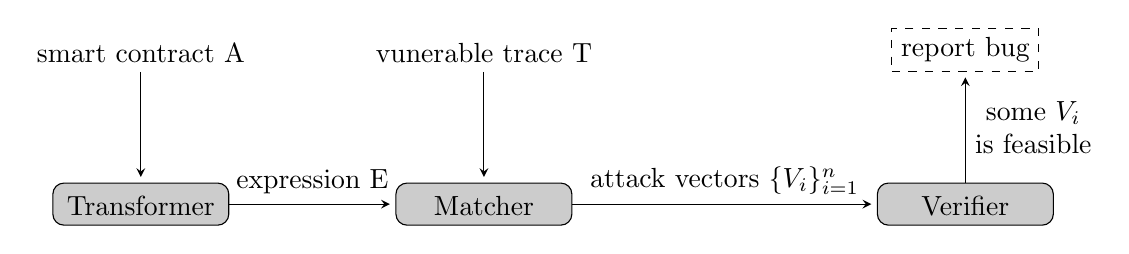
\begin{tikzpicture}[% 	
	every text node part/.style={align=center},
	->,
	shorten >=2pt,
	>=stealth,
	node distance=6em,
	com/.style={%
		rectangle,
		rounded corners,
		fill=gray!40,
		minimum width=3em,
		minimum height=1em,
		align=center,
		draw
	},
	sub/.style={%
		rectangle,
		rounded corners,
		minimum width=3em,
		minimum height=1em,
		draw
	},
	data/.style={%
		rectangle,
		minimum width=3em,
		minimum height=1em,
	},
	res/.style={%
		rectangle,
		dashed,
		minimum width=3em,
		minimum height=1em,
		draw
	}
	] 

	\node[com,text width=2cm, text height = 0.3cm] (transformer){Transformer}; 
	\node[com,text width=2cm, text height = 0.3cm] (matcher)[right=of transformer]{Matcher}; 
	\node[com,text width=2cm, text height = 0.3cm] (verifier)[right=of matcher, xshift=5em]{Verifier};   
	\node[data] (input) [above=of transformer,yshift=-2em] {smart contract A};
	\node[data] (trace)[above=of matcher,yshift=-2em]{vunerable trace T}; 
	\node[res] (result)[above=of verifier,yshift=-2em]{report bug};      
	\draw  (input) -- (transformer);    
	\draw  (trace) -- (matcher);   
	\draw (transformer) --node[data,above] {expression E} (matcher);  
	  \path[every node/.style={}]
	  %(verifier) edge[bend left=30] node[below]  {V is infeasible} (matcher)
    %(matcher) edge[bend left=30] node[above]  {matched with new \\ attack vector %V} (verifier)
    (matcher) edge[above] node {attack vectors $\{V_i\}_{i=1}^n$} (verifier)
    (verifier) edge[right] node {some $V_i$ \\ is feasible} (result);
	\end{tikzpicture}
	\caption{Our framework for checking vulnerabilities in Ethereum smart contracts.}\label{fig:framework}	
\end{figure}

\begin{enumerate}
	\item $\textbf{Transformer}$: transform the smart contract A into an expression E (look like regular expression but we can have guard conditions inside).
	\item $\textbf{Matcher}$: check whether $T \in E$, \emph{i.e.} the trace $T$ satisfies the expression $E$. At the same time, generates attack vectors $V$ which contains function/variable assignments.
	\item $\textbf{Verifier}$: run the smart contract with the give input to see whether the vulnerability can be reproduced. We need this step as our semantics over-approximates the Ethereum semantics.
\end{enumerate}

\subsection{Transformation of smart contracts into expressions}

Let $\mathcal{A}$ be the pre-defined abstraction function that maps statements/function's names into abstract symbols. We define the transformation $\trans_n$ that transform a statement into its respective trace form. We use $n$ as the upper limit for the number of times we can unfold nested functions. As a result, our transformation always terminates. Normally, we use $\trans_1$ for all the vulnerability checks, except reentrancy and gasless send in which we use $\trans_2$.
\begin{figure}
$$
\infer[{[\rname{base}]}]{c \trans_{n} c}{
	\begin{array}{c}
	\textsf{primitive}(c)
	\end{array}}
~~~~~
\infer[{[\rname{if}]}]{\ifs{b}{c_1}{c_2} \trans_{n} \textbf{assert}(b);t_1+\textbf{assert}(!b);t_2}{c_1 \trans_{n} t_1~~~~ c_2 \trans_{n} t_2}
$$
$$
\infer[{[\rname{while}]}]{\whiles{b}{c} \trans_{n} (\textbf{assert}(b);t)^*;\textbf{assert}(!b)}{c \trans_{n} t}
~~~~~~
\infer[{[\rname{seq}]}]{c_1;c_2 \trans_{n} t_1 \nxt t_2}{c_1 \trans_{n} t_1~~~~ c_2 \trans_{n} t_2}
$$
$$
\infer[{[\rname{func}_1]}]{c_f \trans_{0} \epsilon}{}
~~~~~~
\infer[{[\rname{func}_2]}]{c_f \trans_{n} c_f[\{I_f\}t]}{n > 0~~\textsf{lookup}(c_f,\chain) = (c,I_f)~~~c \trans_{n-1} t}
$$
\caption{Trace synthesis}\label{fig:syn}
\end{figure}



Matcher: need to propose variables 1st, then check the syntax first, incrementally. From outer to inner. Then semantics.


\section{Implementation}

\section{Evaluation}

\section{Related work}

\section{Conclusion}

\end{document}
